\section{Durchführung}
\label{sec:Durchführung}

Es sollen einfache periodische Schwingungen in ihre Fourier-Komponenten zerlegt und mit den Theoriewerten verglichen werden.
Danach werden einfache periodische Schwingungen aus ihren Fourier-Komponenten zusammengesetzt und durch einen zeitlchen Verlauf der Summenspannung dokumentiert.

\subsection{Messvorrichtung zur Fourier-Analyse}
\label{sec:Analyse}
Ist der als Signalquelle verwendete Funktionsgenerator durchstimmbar, so kann man bereits mit der sehr einfachen in \ref{fig:abb2} skizzierten Apparatur eine solche Analyse ausführen.
\begin{figure}
  \centering
  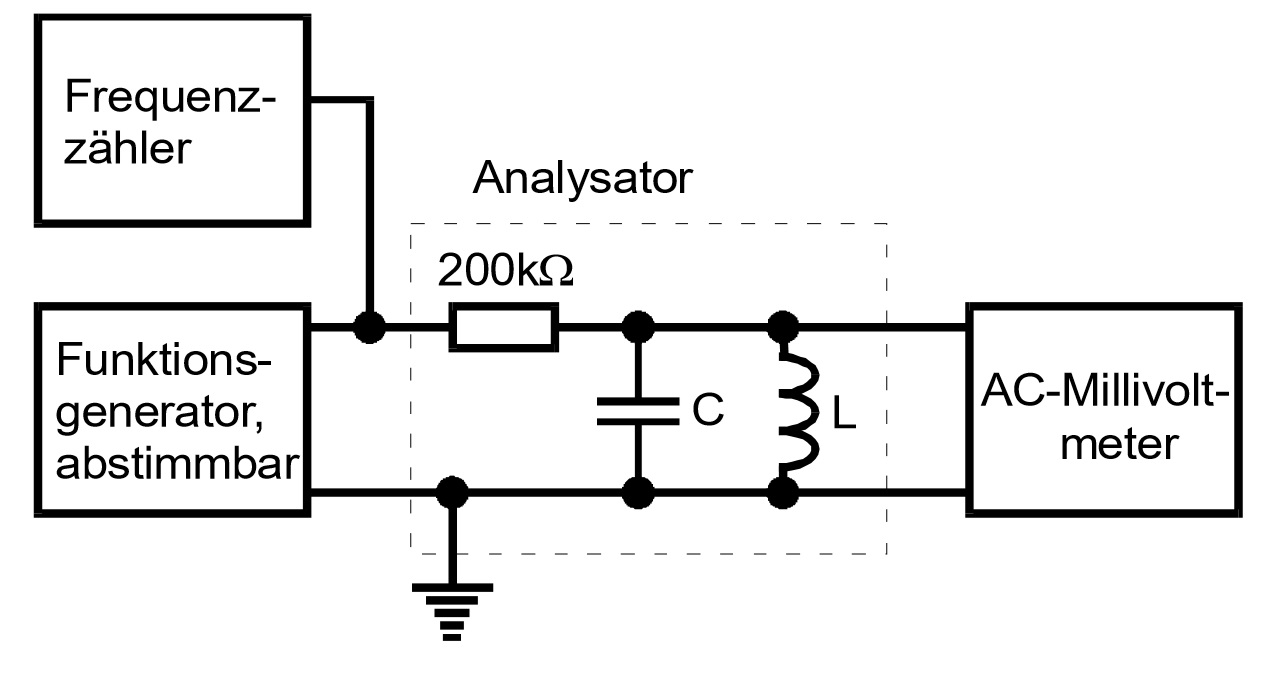
\includegraphics[width=\textwidth]{abb2.jpg}
  \caption{Schaltung zur Fourier-Analyse einer durchstimmbaren Signalquelle.}
  \label{fig:abb2}
\end{figure}
Der Parallelresonanzkreis wird durch die vom Generator erzeugte Signalspannung zu erzwungenen Schwingungen angeregt.
Entspricht eine der Frequenzen im Schwingungsspektrum der Resonanzfrequenz
\begin{align}
  \nu_R = \frac{1}{2 \pi \sqrt{L C}}
\end{align}
des Schwingkreises, so wird durch starke Zunahme der Spannung am Schwingkreis ein Resonnzeffekt verzeichnet.
Durch die Proportionalität der Amplitude der angeregten Oberwelle und der Höhe der Resonanzspannung, kann man das Amplitudenverhältnis der Fourier-Komponenten bestimmen,
indem der LC-Kreis der Reihe nach mit allen Oberwellen angeregt wird.
Die n-te Oberwelle besitzt dann die Frequenzen
\begin{align}
  n \frac{\nu_R}{n} = \nu_R
\end{align}
und bringt den Schwingkreis zur Resonanz.
Während des Messvorgangs muss die Ausgangsamplitude konstant bleiben.
Zum mesen von noch sehr kleinen Fourier-Komponenten, besonders den Wert 0, ist es wichtig eine Resonanzkurve mit sehr steil abfallende Flanken zu haben.
Durch eine Kombination mehrerer Schwingkreise ist es möglich, dass die Abnahme eine Abhängigkeit von $\nu^n$ (n > 2) zu bekommen, an Stelle von $\nu^2$ bei nur einem Schwingkreis.

\subsection{Fourier-Synthese}
\label{sec:Synthese}
Umgekehrt kann man, wenn man die einzelnen Fourier-Komponenten einer Schwingung kennt diese schrittweise aus ihren Komponenten zusammensetzen und beobachten, wie genau die endliche Fourier-Summe die Gesuchte Kurve annähert.
Hierzu wird ein Siganlgenerator , der Sinusschwingungen der Frequenzen $\nu$, $2 \nu$, $3 \nu$, .... mit beliebig einstellbaren Amplituden liefert verwendet.
Die Phasen müssen zeitlich konstant sein und dürfen lediglich die Werte $0$, $\pi / 2$ und $3 \pi / 2$ annhemen, falls f(t) weder gerade noch ungerade ist.
Sonst genügen $0$ und $\pi$.
Durch schrittweises addieren der Fourier-Komponenten kann das Ergebnis auf dem Bildschirm eines Oszilloskops sichtbar gemacht werden.

\subsection{Fourier-Analyse mittels Fourier-Transformation}
\label{sec:Analyse durch Transormation}
Es wird wiederum ein Funktionsgenerator als Signalquelle verwendet, dessen Frequenz aber im Gegensatz zu dem in \ref{sec:Analyse} beschriebenen Verfahren konstant bleibt.
Hier wird die Fourier-Transformation von einem Rechner ausgeführt.
Dafür wird das Siganl auf ein Analaog-Digital-Konverter gegeben.
Somit hat das vereinfachte Schaltbild die in \ref{fig:abb3} dargestellte Gestallt.
\begin{figure}
  \centering
  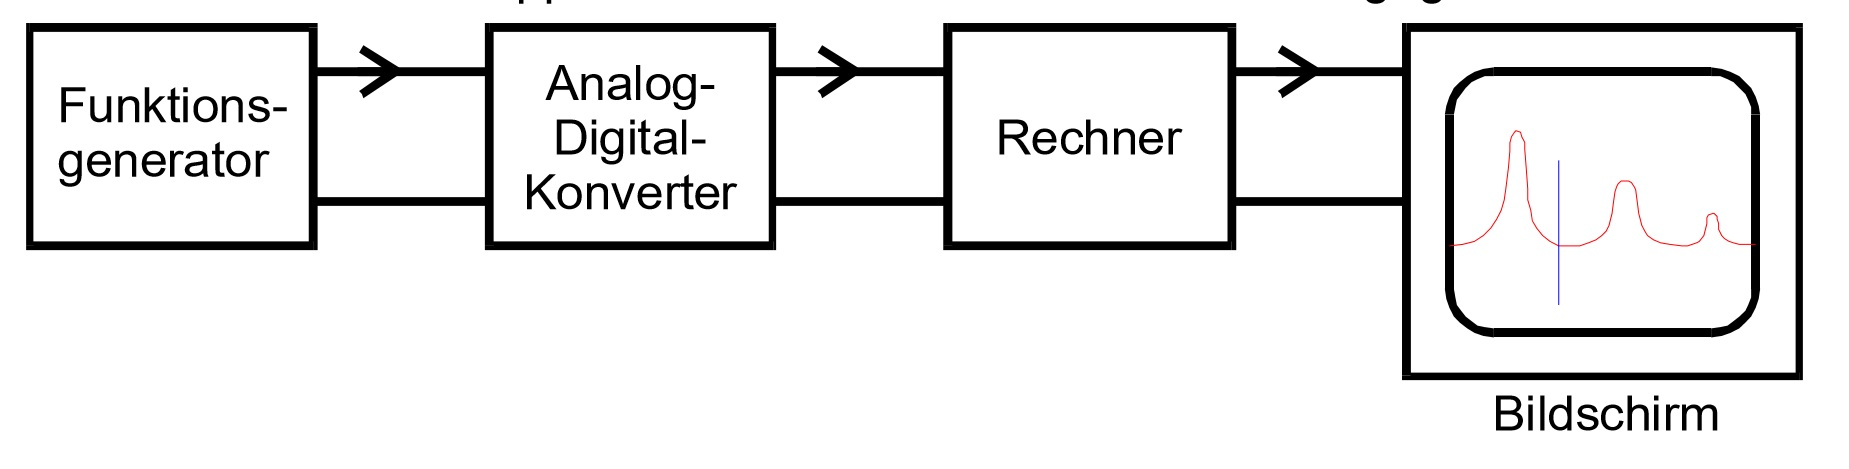
\includegraphics[width=\textwidth]{abb3.jpg}
  \caption{Schematische Darstellung der auf der Grundlage der Fourier-Transformation arbeitenden Messaparatur.}
  \label{fig:abb3}
\end{figure}
Weil der Analaog-Digital-Konverter nur in endlichen Zeitabständen einen Spannungswert nehmen kann kann die Funktion f(t) nicht kontinuierlich aufgezeichnet werden,
sondern nur durch diskrete Messpunkte dargestellt werden.
Sind die Zeitabstände verglichen mit der Periodendauer von f zu groß, dann kann die Funktion aus den wenigen Punkten pro Periode nicht rekonstruiert werden und es kommt zu gewaltigen Fehlern.
Man kann jedoch nachweisen, dass der Fehler vernachlässigbar klein wird, wenn die Abstandsfrequenz $\nu_A$ größer als das doppelte der größten im Spektrum von f vorkommenden Frequenz ist
\begin{equation}
  \nu_A > 2 \nu_{max}
  \label{eqn:gl4}
\end{equation}
Die Ungleichung \ref{eqn:gl4} bezeichnet man als Abstandstheorem.
Der Rechner führt die Fourier-Transformation durch und trägt die Signalspnnung in Abhängigkeit von der Zeit auf.
Die Integration wird nach der Simpson-Regel ausgeführt und es wird der Betrag von g als
\begin{align}
  |g| = \sqrt{Re^2 (g) + Im^2 (g)}
\end{align}
berechnet.
Dann kann man, in Abhängigkeit von der Frequenz, $|g|$ für einzelne Komponenten oder mehrere Oberwellen und ihre Amplituden $|g(\nu_i)|$ bestimmen.\cite{AnleitungV351}
